%%% Copyright (C) 2020 David Beauchemin
%%%
%%% Ce fichier et tous les fichiers .tex dont la racine est
%%% mentionnée dans les commandes \include et \input ci-dessous font
%%% partie du projet «Reproductibilité en apprentissage automatique
%%% - Webinaire de l'institut intelligence et données»
%%% https://davebulaval.github.io/reproductibilite-en-apprentissage-automatique/
%%%
%%% Le format et le visuel est très fortement inspiré du matériel de
%%% Vincent Goulet https://gitlab.com/vigou3/webinaire-recherche-reproductible
%%%
%%% Cette création est mise à disposition selon le contrat
%%% Attribution-Partage dans les mêmes conditions 4.0
%%% International de Creative Commons.
%%% https://creativecommons.org/licenses/by-sa/4.0/

\documentclass[aspectratio=169,10pt,xcolor=x11names,english,french]{beamer}
\usepackage{babel}
\usepackage[autolanguage]{numprint}
\usepackage{amsmath}
\usepackage{currfile}                  % nom fichier de script
\usepackage{changepage}                % page licence
\usepackage{tabularx}                  % page licence
\usepackage{relsize}                   % \smaller et al.
\usepackage{awesomebox}                % boites signalétiques
\usepackage{fancyvrb}                  % texte verbatim
\usepackage{framed}                    % env. leftbar
\usepackage{pict2e}                    % cycle travail Git
\usepackage[overlay,absolute]{textpos} % couvertures
\usepackage{metalogo}       
\usepackage{textpos}           % logo \XeLaTeX

\usepackage{fontawesome}

\usepackage{stackengine, tikz} % for stacking logo

\usepackage{svg} %for svg image also need option --shell-escape

%% =============================
%%  Informations de publication
%% =============================
\title{Reproductibilité en apprentissage automatique}
\author{David Beauchemin}
\date{30 octobre 2020}

%% =======================
%%  Apparence du document
%% =======================

%% Thème Beamer général
\usetheme[titleformat=allcaps, numbering=none, block=transparent]{metropolis}

%% Modifications aux couleurs: fond blanc, titres en texte noir sur
%% fond blanc
\setbeamercolor{normal text}{bg=white}
\setbeamercolor{frametitle}{fg=normal text.fg, bg=}

%% Déplacer les titres vers le bas sous la décoration du gabarit CFDD
\makeatletter
\setlength{\metropolis@frametitle@padding}{4.9ex}
\renewcommand{\metropolis@frametitlestrut@start}{
	\rule{0pt}{6ex +%
		\totalheightof{%
			\ifcsdef{metropolis@frametitleformat}{\metropolis@frametitleformat X}{X}%
		}%
	}
}
\renewcommand{\metropolis@frametitlestrut@end}{}
\makeatother

%% Format de la page de titre de section;
\makeatletter
\setbeamertemplate{section page}{%
	\begin{textblock*}{92.5mm}[1,1](187mm,90mm)
		
\includegraphics[height=\paperheight,keepaspectratio, angle=180,origin=c]{img/degrade-coin-rouge}
	\end{textblock*}
	\begin{minipage}{22em}
		\raggedright
		\usebeamerfont{section title}
		\let\hyperlink\@secondoftwo\textcolor[cmyk]{0.67, 0.66, 0, 0.71}{\insertsectionhead}\par
	\end{minipage}
	\par
	\vspace{\baselineskip}
}
\makeatother

%% Polices de caractères
\newfontfamily\Overpass{Overpass}
\setsansfont{Overpass}        % police principale
\newfontfamily\OverpassSemiBold{Overpass}
[
BoldFont = *-SemiBold
]
\newfontfamily\OverpassExtraLightBold{Overpass}
[
UprightFont = *-ExtraLight,
BoldFont = *-Light
]
\newfontfamily\OverpassLight{Overpass}
[
UprightFont = *-Light,
BoldFont = *-Regular
]

%% Couleurs additionnelles
\definecolor{comments}{cmyk}{0,1, 1, 0}   % rouge foncé
\definecolor{link}{cmyk}{0.67, 0.66, 0, 0.71}    % liens internes
\definecolor{url}{cmyk}{0,1, 1, 0}       % liens externes
\definecolor{codebg}{named}{LightYellow1} % fond code R
\definecolor{rouge}{rgb}{0.85,0,0.07} % bandeau rouge UL
\definecolor{or}{rgb}{1,0.8,0}        % bandeau or UL
\definecolor{couleurpolice}{cmyk}{0.67, 0.66, 0, 0.71}

\colorlet{alert}{mLightBrown} % alias pour couleur Metropolis
\colorlet{dark}{mDarkTeal}    % alias pour couleur Metropolis
\colorlet{code}{mLightGreen}  % alias pour couleur Metropolis
\colorlet{shadecolor}{codebg}


\setbeamercolor{frametitle}{fg=couleurpolice}
\setbeamercolor{section in head/foot}{fg=couleurpolice}
\setbeamercolor{normal text}{fg=couleurpolice}



%% Hyperliens
\hypersetup{%
	pdfauthor = {David Beauchemin},
	pdftitle = {Reproductibilité en apprentissage automatique},
	colorlinks = {true},
	linktocpage = {true},
	allcolors = {link},
	urlcolor = {url},
	pdfpagemode = {UseOutlines},
	pdfstartview = {Fit},
	bookmarksopen = {true},
	bookmarksnumbered = {true},
	bookmarksdepth = {subsection}}

%% Paramétrage de babel pour les guillemets
\frenchbsetup{og=«, fg=»}

%% =========================
%%  Nouveaux environnements
%% =========================

%% Environnement pour le code informatique; hybride
%% des environnements snugshade* et leftbar de framed.
\makeatletter
\newenvironment{Scode}{%
	\def\FrameCommand##1{\hskip\@totalleftmargin
		\vrule width 3pt\colorbox{codebg}{\hspace{5pt}##1}%
		% There is no \@totalrightmargin, so:
		\hskip-\linewidth \hskip-\@totalleftmargin \hskip\columnwidth}%
	\MakeFramed {\advance\hsize-\width
		\@totalleftmargin\z@ \linewidth\hsize
		\advance\labelsep\fboxsep
		\@setminipage}%
}{\par\unskip\@minipagefalse\endMakeFramed}
\makeatother

%% Environnement pour le contenu d'un fichier; alias de snugshade*.
\newenvironment{Sfile}{\begin{snugshade*}}{\end{snugshade*}}

%% =====================
%%  Nouvelles commandes
%% =====================

%% Lien externe
\newcommand{\link}[2]{\href{#1}{#2~{\smaller\faExternalLink*}}}

%% Simili commande \HUGE
\newcommand{\HUGE}{\fontsize{36}{36}\selectfont}

%% Raccourcis usuels vg
\newcommand{\code}[1]{\textcolor{code}{\texttt{#1}}}

%%% =======
%%%  Varia
%%% =======

%% Longueurs pour la composition des pages couvertures avant et
%% arrière
\newlength{\banderougewidth} \newlength{\banderougeheight}
\newlength{\bandeorwidth}    \newlength{\bandeorheight}
\newlength{\imageheight}     \newlength{\imagewidth}
\newlength{\logoheight}

\begin{document}
	
	%% Style de l'entête et du pied de page
	
	%% frontmatter
	%%% Copyright (C) 2020 David Beauchemin
%%%
%%% Ce fichier et tous les fichiers .tex dont la racine est
%%% mentionnée dans les commandes \include et \input ci-dessous font
%%% partie du projet «Reproductibilité en apprentissage automatique
%%% - Webinaire de l'AAIARD»
%%% https://davebulaval.github.io/reproductibilite-en-apprentissage-automatique/
%%%
%%% Le format et le visuel est très fortement inspiré du matériel de
%%% Vincent Goulet https://gitlab.com/vigou3/webinaire-recherche-reproductible
%%%
%%% Cette création est mise à disposition selon le contrat
%%% Attribution-Partage dans les mêmes conditions 4.0
%%% International de Creative Commons.
%%% https://creativecommons.org/licenses/by-sa/4.0/

%% Normes de présentation visuelle 2018
%%
%% - grille de 8 unités de haut
%% - 1 mesure = 1/8 d'unité
%% - bande identitaire de 1 mesure placée au bas de la 7e unité
%% - logo haut de 4 mesures avec blancs de deux mesures en haut et
%%   en bas
%% - blanc équivalent à la largeur du blason à droite du logo
%% - bande or de la largeur du logo + blanc à droite
%%
%% Dimensions du logo UL
%%
%% hauteur: 129
%% largeur totale: 312
%% largeur blason: 102
%% valeur clé: (312 + 102)/129 = 3.209302
%%
%% Dimensions de l'image
%%
%% hauteur: 55 mesures - 1pt (filet) = 54.9191919 mesures
%% largeur: 160mm
%% ratio largeur/hauteur: 160/77.23

\begingroup
\TPGrid{16}{64}
\textblockorigin{0mm}{0mm}
\setlength{\parindent}{0mm}
\setlength{\imageheight}{54.9191919\TPVertModule}
\setlength{\logoheight}{4\TPVertModule}
\setlength{\bandeorwidth}{3.209302\logoheight}
\setlength{\banderougewidth}{\paperwidth}
\addtolength{\banderougewidth}{-\bandeorwidth}
\setlength{\bandeorheight}{\TPVertModule}
\setlength{\banderougeheight}{\TPVertModule}
\setlength{\textwidth}{\paperwidth}
\addtolength{\textwidth}{-2\TPHorizModule}

\def\titlefmt{%
  \bfseries\fontsize{24}{24}\selectfont%
  REPRODUCTIBILITÉ EN \\APPRENTISSAGE AUTOMATIQUE\par}
\def\webinaire{%
  \OverpassSemiBold\bfseries\fontsize{18}{18}\selectfont
  WEBINAIRE}
\def\datefmt{%
  \OverpassExtraLightBold\bfseries\fontsize{14}{14}\selectfont%
  15 DÉCEMBRE 2020}

%%%
%%% Page de titre
%%%
\begin{frame}[plain]
	%% bandeau identitaire
	\begin{textblock*}{\paperwidth}[0,1](0mm,56\TPVertModule)
		\textcolor{rouge}{\rule{\banderougewidth}{\banderougeheight}}%
		\textcolor{bleu}{\rule{\bandeorwidth}{\bandeorheight}}
	\end{textblock*}
	
	%% identifiant «webinaire»
	\begin{textblock*}{2\TPHorizModule}(0.7\TPHorizModule,5\TPVertModule)
		\textcolor[rgb]{0.13,0.13,0.13}{\webinaire}
	\end{textblock*}
	
	%% titre
	\begin{textblock*}{12\TPHorizModule}(0.7\TPHorizModule,17\TPVertModule)
		\textcolor[rgb]{0.13,0.13,0.13}{\titlefmt}
	\end{textblock*}
	
	%% date
	\begin{textblock*}{10\TPHorizModule}(0.7\TPHorizModule,41\TPVertModule)
		\textcolor[rgb]{0.13,0.13,0.13}{\datefmt}
	\end{textblock*}
\end{frame}
\endgroup

	
	\begin{frame}{Objectifs de la présentation}
		\begin{itemize}
			\item Inciter l'intégration des solutions permettant une meilleure reproductibilité dans vos solutions d'affaires et académiques.
			\item Améliorer la reproductibilité de vos projets.
			\item Améliorer votre productivité.
		\end{itemize}
	\end{frame}
	
	\begin{frame}
		\frametitle{Votre conférencier}
		
		\begin{minipage}{0.25\linewidth}
			
\includegraphics[width=\linewidth,keepaspectratio]{img/david}
		\end{minipage}
		\hfill
		\begin{minipage}{0.70\linewidth}
			\begin{itemize}
				\item Introduit à la recherche reproductible en 2016 (\mbox{R Markdown} et \faGit)
				\item Participation à REPROLANG de la conférence LREC \cite{garneau2020robust}
				\item Membre actif dans le développement d'une librairie facilitant la reproductibilité (\href{https://poutyne.org/}{Poutyne})
			\end{itemize}
		\end{minipage}
		
		\begin{minipage}{0.25\linewidth}
			\small
			\textbf{DAVID BEAUCHEMIN} \\
			Candidat au doctorat \\
			Département d'informatique et de génie logiciel
		\end{minipage}
	\end{frame}

	\begin{frame}{Au menu}
		\begin{minipage}{0.24\linewidth}
				\centering
				\fontsize{35}{35}\faFilesO \vfil
				\vspace{1em}
				\normalsize Gestion version
		\end{minipage}
		\begin{minipage}{0.24\linewidth}
				\centering
				\fontsize{35}{35}\faTachometer\vfil
				\vspace{1em}
				\normalsize Productivité
				
		\end{minipage}
		\begin{minipage}{0.24\linewidth}
				\centering
				% Camille comment : Cette icone a un problème d'alignement ... 
				\fontsize{35}{35}\faPencilSquareO\vfil
				\vspace{1em}
				\normalsize Présenter
		\end{minipage}
		\begin{minipage}{0.24\linewidth}
				\centering
				\fontsize{35}{35}\faRecycle\vfil
				\vspace{1em}
				\normalsize Réutiliser
		\end{minipage}
	\end{frame}
	
	\section{Introduction}
	\begin{frame}{C'est quoi la reproductibilité ?}
		La reproductibilité est le principe qui dit qu'on ne peut tirer de conclusions que d'un événement bien décrit, qui est apparu plusieurs fois, provoqué par des \textbf{personnes différentes}.
		
		Par contre, en apprentissage automatique, la reproductibilité correspond (surtout) soit à être capable de reproduire des résultats, soit d'obtenir des résultats similaires en réexécutant un code source\cite{pineau2020improving}.
		
		\note{
			
			Être capable de \textbf{répliquer} les résultats d'un article d'un projet, 
			
			à partir du même \textbf{jeu de données} ou un jeu de données différent (mais proche), 
			
			en utilisant la \textbf{procédure d'entraînement} de l'article ou en utilisant notre procédure d'entrainement et 
			
			en utilisant le \textbf{code} du projet.
			
			les points clés c'est l'idée que si une idée a de bons résultats, on devrait être capable de la reprendre et de retrouver les mêmes résultats.
			
			En ML, les idées c'est des algos et la reproductibilité devient juste d'être capable de s'assurer que les performances rapportées sont les mêmes.
				
	}
	\end{frame}
	
	\begin{frame}{Pourquoi s'y intéresser ?}
		\centering
		\fontsize{35}{35}\selectfont70~\%\fontsize{25}{25}\footnote[1]{\cite{baker500ScientistsLift2016}}
		
		\note{
			$70$~\% des chercheurs en science on échoué dans leur tentative de reproduire un article d'un autre chercheur
		}
	\end{frame}

	\begin{frame}{Pourquoi s'y intéresser ?}
	\centering
	\fontsize{35}{35}\selectfont50~\%\fontsize{25}{25}\footnote[1]{\cite{baker500ScientistsLift2016}}

		
		\note{
			$50$~\% n'ont pas réussit à reproduire leurs \textbf{propres} expérimentations
		}
	
	\end{frame}

	\begin{frame}{Pourquoi s'y intéresser ?}
		\centering
		\fontsize{35}{35} \selectfont40~\%\fontsize{25}{25}\footnote[2]{\cite{raff2019step}}
		
		
		\note{
			L'informatique ne fait pas exception à cela malgré la simplicité (théorique) de réplication des résultats. Selon une étude, sur \textbf{255} articles, près de $40$~\% n'étaient pas réplicable \cite{raff2019step}.
		}
		
	\end{frame}
	
	\begin{frame}{Motivation}
		\centering
		\uncover<1->{\begin{minipage}{0.24\linewidth}
				\centering
				\fontsize{35}{35}\faRecycle\vfil
				\vspace{1em}
				\normalsize Réutilisation
		\end{minipage}}
		\uncover<2->{\begin{minipage}{0.24\linewidth}
				\centering
				\fontsize{35}{35}\faForward\vfil
				\vspace{1em}
				\normalsize Productivité
		\end{minipage}}
		\uncover<3->{\begin{minipage}{0.24\linewidth}
				\centering
				\fontsize{35}{35}\faShare\vfil
				\vspace{1em}
				\normalsize Transfert
		\end{minipage}}
		\uncover<4->{\begin{minipage}{0.24\linewidth}
				\centering
				\fontsize{35}{35}\faMapPin\vfil
				\vspace{1em}
				\normalsize Se faire connaître
		\end{minipage}}
		\note{La reproductibilité facilite la \textbf{réutilisation} pour d'autres projets de recherche, améliorer votre productivité \textbf{et} permet le transfert vers l'industrie (plus facilement). En bonus, cela aide à vous faire connaître si vous faites du contenu réutilisable par la communauté.}
	\end{frame}
	
	\section{Les barrières à la reproductibilité}
%		\begin{frame}		\def\ban{\fontsize{65}{65}\selectfont\textcolor[cmyk]{0.67, 0.66, 0, 0.71}\faBan}
%		\def\database{\fontsize{35}{35}\selectfont\textcolor[cmyk]{0.67, 0.66, 0, 0.71}\faDatabase}
%		\def\code{\fontsize{35}{35}\selectfont\textcolor[cmyk]{0.67, 0.66, 0, 0.71}\faCode}
%		\def\gear{\fontsize{35}{35}\selectfont\textcolor[cmyk]{0.67, 0.66, 0, 0.71}\faCog}
%		\centering
%		\uncover<1->{\begin{minipage}{0.24\linewidth}
%			\centering
%			\def\stackalignment{c}
%			\topinset{\database}{\rotatebox{90}{\ban}}{14pt}{-1pt}\vfil
%			\vspace{1em}
%			\normalsize Non-disponibilité des données
%		\end{minipage}}
%		\uncover<2->{\begin{minipage}{0.24\linewidth}
%				\centering
%				% Camille : encore le facogs qui gosse
%				\fontsize{35}{35}\selectfont\textcolor[cmyk]{0.67, 0.66, 0, 0.71}\faCogs\vfil
%				\vspace{1em}
%				\normalsize Mauvaise spécification
%		\end{minipage}}
%		\uncover<3->{\begin{minipage}{0.24\linewidth}
%				\centering
%				\def\stackalignment{c}
%				\topinset{\code}{\rotatebox{90}{\ban}}{14pt}{-1pt}\vfil
%				\vspace{1em}
%				\normalsize Non-disponibilité du code
%		\end{minipage}}
%		\uncover<4->{\begin{minipage}{0.24\linewidth}
%				\centering
%				\def\stackalignment{c}
%				\topinset{\gear}{\rotatebox{90}{\ban}}{14pt}{-1pt}\vfil
%				\vspace{1em}
%				\normalsize Non-disponibilité des configurations
%		\end{minipage}}
%	\note{Non-disponibilité du jeu de données ou \textbf{version} (pas claire) du jeu de données, 
%		\textbf{mauvaise spécification ou sous-spécification} du modèle et de la \textbf{procédure d'entraînement},
%		manque de \textbf{disponibilité du code} nécessaire pour exécuter les expériences, ou \textbf{erreurs} dans le code,
%		\textbf{configurations} du modèle déficientes
%	}
%	\end{frame}
	
	\begin{frame}
		\begin{figure}
			\centering
			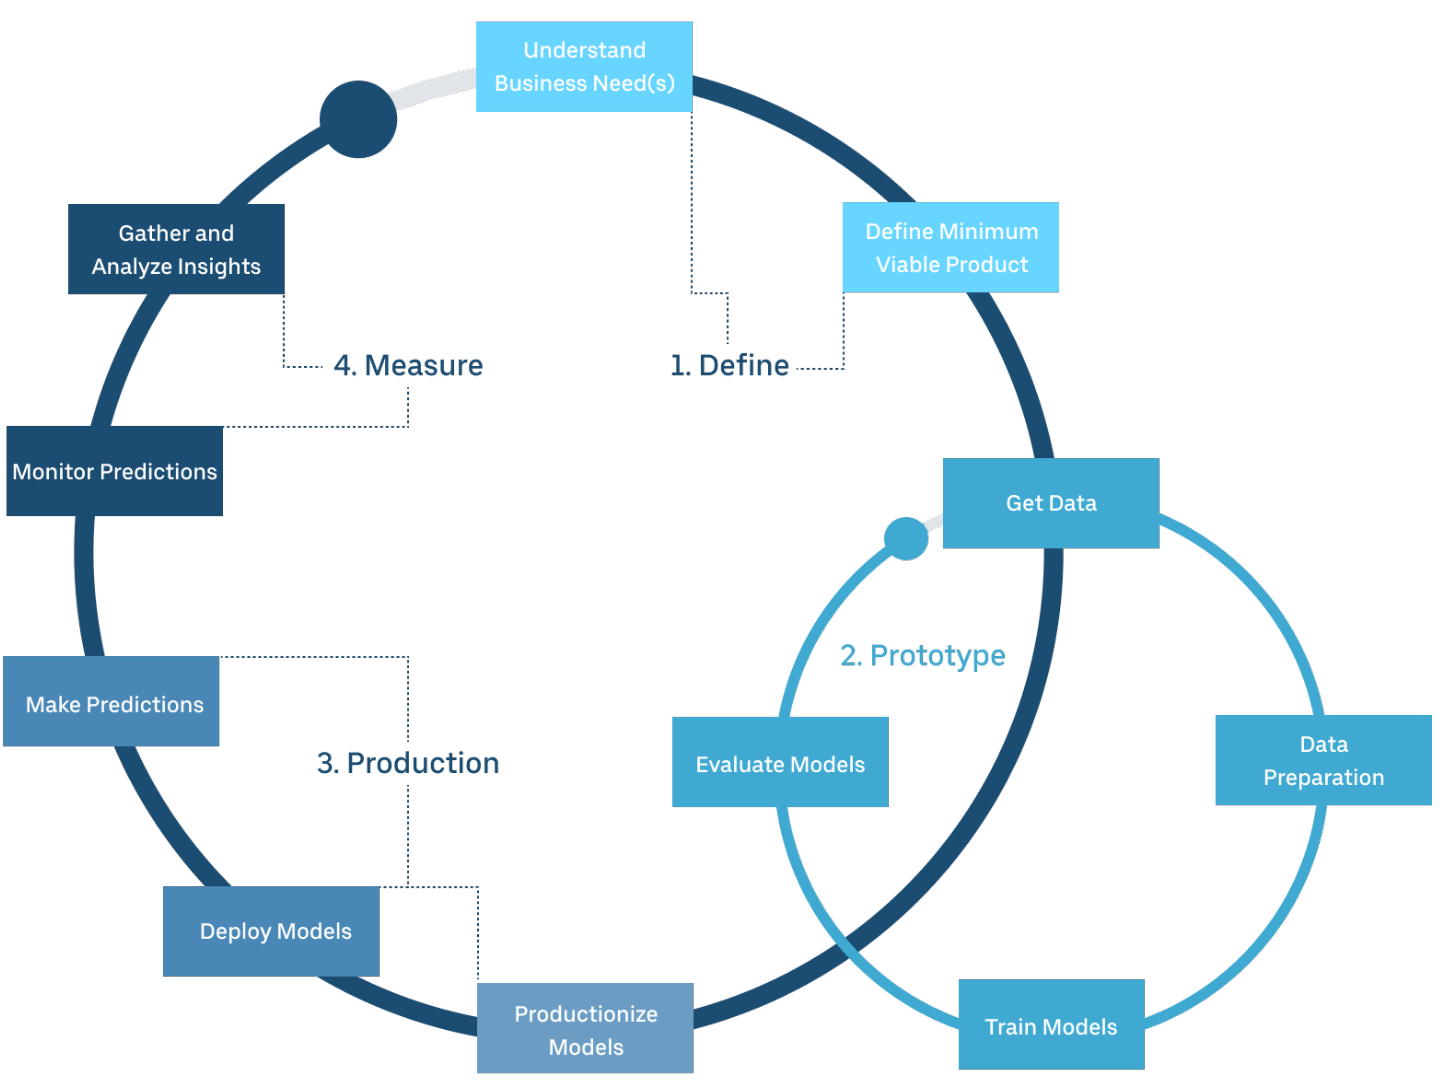
\includegraphics[scale=0.19]{img/cycle.png}
			\caption{\href{https://eng.uber.com/scaling-michelangelo/}{From Uber Engineering}}
		\end{figure}
	\end{frame}
	
	\begin{frame}
		\begin{figure}
			\centering
			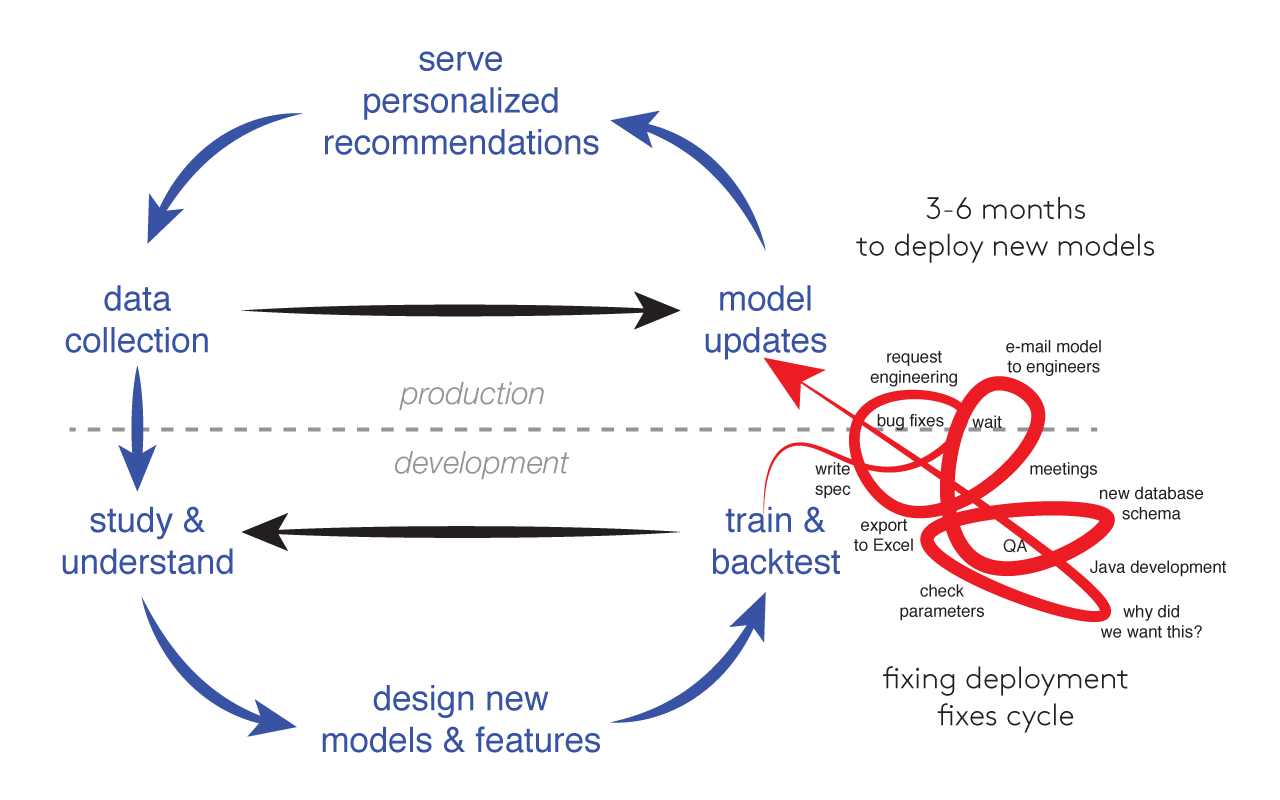
\includegraphics[scale=0.24]{img/cycle-white.png}
			\caption{\href{https://johann.schleier-smith.com/blog/2015/08/09/need-for-agile-machine-learning.html}{The need for Agile machine learning}}
		\end{figure}
	\end{frame}
	
	\section{OK, mais comment?}
	
	\begin{frame}{Au menu}
		\begin{minipage}{0.24\linewidth}
			\centering
			\fontsize{35}{35}\faFilesO
			\vfil
			\vspace{1em}
			\normalsize Gestion version
		\end{minipage}
		\begin{minipage}{0.24\linewidth}
			\centering
			\tikz\node[opacity=0.5]{\fontsize{35}{35}\faTachometer};
			\vfil
			\vspace{1em}
			\tikz\node[opacity=0.5]{\normalsize Productivité};
			
		\end{minipage}
		\begin{minipage}{0.24\linewidth}
			\centering
			\tikz\node[opacity=0.5]{\fontsize{35}{35}\faPencilSquareO};
			\vfil
			\vspace{1em}
			\tikz\node[opacity=0.5]{\normalsize Présenter};
		\end{minipage}
		\begin{minipage}{0.24\linewidth}
			\centering
			\tikz\node[opacity=0.5]{\fontsize{35}{35}\faRecycle};
			\vfil
			\vspace{1em}
			\tikz\node[opacity=0.5]{\normalsize Réutiliser};
		\end{minipage}
	\end{frame}

	\begin{frame}{Version des données \& Étapes de prétraitement}
		\centering
		\uncover<1->{\begin{minipage}{0.32\linewidth}
				\centering
				\fontsize{35}{35}\faCopy\vfil
				\vspace{1em}
				\normalsize Version
		\end{minipage}}
		\uncover<2->{\begin{minipage}{0.32\linewidth}
				\centering
				\fontsize{35}{35}\faServer\vfil
				\vspace{1em}
				\normalsize Gestion des versions
		\end{minipage}}
		\uncover<3->{\begin{minipage}{0.32\linewidth}
				\centering
				\fontsize{35}{35}\faRoad\vfil
				\vspace{1em}
				\normalsize Étapes prétraitement
		\end{minipage}}
		\note{
			Avec quelle version des données doit-on travailler?
			
			Comment gérer \textbf{facilement} plusieurs versions des données?
			
			Comment définir \textbf{facilement} les étapes de prétraitement des données?
			
			Il nous faut des \textit{\textbf{data pipelines}}, des tuyaux que nous pouvons \textbf{facilement} raccorder à nos modèles pour l'entrainement et la mise en production.
		
			Il faut somewhat voir nos données comme du code et qu'à chaque fois qu'on fait du traitement sur notre data c'est comme modifier notre codebase et c'est impératif d'avoir une trace, par exemple ...
		}
		
	\end{frame}

	\begin{frame}{Version des données \& Étapes de prétraitement}
		\begin{minipage}{0.49\linewidth}
			\centering
			\includesvg[width=40pt, height=40pt]{./img/DVC} \vfil
			\vspace{1.25em}
			\href{https://dvc.org/}{Data Version Control}
		\end{minipage}
			\begin{minipage}{0.49\linewidth}
				\centering
				\includesvg[width=30pt, height=30pt]{./img/dask} \vfil
				\vspace{0.75em}
				\href{https://dask.org/}{Dask}
			\end{minipage}
 	\end{frame}
	
	\begin{frame}{Code}
		\uncover<1->{\begin{minipage}{0.32\linewidth}
				\centering
				\fontsize{35}{35}\faCopy\vfil
				\vspace{1em}
				\normalsize Version
		\end{minipage}}
		\uncover<2->{\begin{minipage}{0.32\linewidth}
				\centering
				\fontsize{35}{35}\faList\vfil
				\vspace{1em}
				\normalsize Différence
		\end{minipage}}
		\uncover<3->{\begin{minipage}{0.32\linewidth}
				\centering
				\fontsize{35}{35}\faCodeFork\vfil
				\vspace{1em}
				\normalsize Divergences
		\end{minipage}}
		\note{
			Avec quelle version du code doit-on travailler?
			
			Comment savoir \textbf{rapidement} qu'elle est la différence d'implémentation entre deux versions du modèle?
			
			Comment gérer \textbf{facilement} les divergences d'expérimentations?
			
			Il nous faut un outil nous permettant de \textbf{visualiser} la différence entre des fichiers de code et nous permettant d'avoir \textbf{plusieurs} versions du code en même temps, par exemple ...
		}
	\end{frame}

	\begin{frame}{Code}
		\begin{minipage}{0.24\linewidth}
			\centering
			\fontsize{35}{35}\faGit\vfill
			\vspace{1em}
			\normalsize \href{https://git-scm.com/}{Git}
		\end{minipage}
		\begin{minipage}{0.24\linewidth}
			\centering
			\fontsize{35}{35}\faGithub\vfill
			\vspace{1em}
			\normalsize \href{https://github.com/}{GitHub}
		\end{minipage}
		\begin{minipage}{0.24\linewidth}
			\centering
			\fontsize{35}{35}\faGitlab\vfill
			\vspace{1em}
			\normalsize \href{https://gitlab.com/}{GitLab}
		\end{minipage}
		\begin{minipage}{0.24\linewidth}
			\centering
			\fontsize{35}{35}\faBitbucket\vfill
			\vspace{1em}
			\normalsize \href{https://bitbucket.org/}{Bitbucket}
		\end{minipage}
	\end{frame}

	\begin{frame}{Au menu}
		\begin{minipage}{0.24\linewidth}
			\centering
			\tikz\node[opacity=0.5]{\fontsize{35}{35}\faFilesO};
			\vfil
			\vspace{1em}
			\tikz\node[opacity=0.5]{\normalsize Gestion version};
		\end{minipage}
		\begin{minipage}{0.24\linewidth}
			\centering
			\fontsize{35}{35}\faTachometer
			\vfil
			\vspace{1.5em}
			\normalsize Productivité
			
		\end{minipage}
		\begin{minipage}{0.24\linewidth}
			\centering
			\tikz\node[opacity=0.5]{\fontsize{35}{35}\faPencilSquareO};
			\vfil
			\vspace{1em}
			\tikz\node[opacity=0.5]{\normalsize Présenter};
		\end{minipage}
		\begin{minipage}{0.24\linewidth}
			\centering
			\tikz\node[opacity=0.5]{\fontsize{35}{35}\faRecycle};
			\vfil
			\vspace{1em}
			\tikz\node[opacity=0.5]{\normalsize Réutiliser};
		\end{minipage}
	\end{frame}
	
	\subsection{Développement}
	\begin{frame}{Développement des modèles}
		\def\ban{\fontsize{65}{65}\faBan}
		\def\tool{\fontsize{35}{35}\faWrench}
		\centering
		\uncover<1->{\begin{minipage}{0.32\linewidth}
				\centering
				\def\stackalignment{c}
				\topinset{\tool}{\rotatebox{90}{\ban}}{14pt}{-1pt}\vfil
				\vspace{1em}
				\normalsize Réinventer
		\end{minipage}}
		\uncover<2->{\begin{minipage}{0.32\linewidth}
				\centering
				% Camille : Celui la aussi il a pas la même taille initiale.
				\fontsize{35}{35}\faMinusSquareO\vfil
				\vspace{3.5em}
				\normalsize Simplification
		\end{minipage}}
		\uncover<3->{\begin{minipage}{0.32\linewidth}
				\centering
				\fontsize{35}{35}\faForward\vfil
				\vspace{3.5em}
				\normalsize Facilite
		\end{minipage}}
		\note{
			Ne pas réinventer la roue.
			
			Simplifier l'écriture de code pour développer des modèles.
			
			Qui facilite l'entrainement (GPU, multi-GPU/CPU).
			
			Il nous faut des outils nous permettant de \textbf{simplifier} le \textbf{développement} de nos modèles, par exemple ...
		}
	\end{frame}

	\begin{frame}{Développement des modèles}
		\begin{minipage}{0.19\linewidth}
			\centering
			\includesvg[width=40pt, height=40pt]{./img/poutyne} \vfil
			\vspace{1.5em}
			\href{https://poutyne.org/}{Poutyne}
		\end{minipage}
		\begin{minipage}{0.19\linewidth}
			\centering
			\includesvg[width=40pt, height=40pt]{./img/lightning} \vfil
			\vspace{2.75em}
			\href{https://www.pytorchlightning.ai/}{PyTorch Lightning}
		\end{minipage}
		\begin{minipage}{0.19\linewidth}
			\centering
			\includesvg[width=40pt, height=40pt]{./img/scikitlearn} \vfil
			\vspace{2.75em}
			\href{https://scikit-learn.org/stable/}{Scikit-learn}
		\end{minipage}
			\begin{minipage}{0.19\linewidth}
				\centering
				\includesvg[width=40pt, height=40pt]{./img/gensim} \vfil
				\vspace{1em}
				\href{https://radimrehurek.com/gensim/}{Gensim}
			\end{minipage}
			\begin{minipage}{0.19\linewidth}
				\centering
				\includesvg[width=40pt, height=40pt]{./img/AllenNLP} \vfil
				\vspace{3.75em}
				\href{https://github.com/allenai/allennlp}{Allen NLP}
			\end{minipage}
	\end{frame}
	
	
	\begin{frame}{Entraînement, configuration et résultats}
		\centering
		\uncover<1->{\begin{minipage}{0.24\linewidth}
				\centering
				\fontsize{35}{35}\faCodeFork\vfil
				\vspace{1em}
				\normalsize Version de l'entraînement
		\end{minipage}}
		\uncover<2->{\begin{minipage}{0.24\linewidth}
				\centering
				\fontsize{35}{35}\faAreaChart\vfil
				\vspace{1em}
				\normalsize Résultats
		\end{minipage}}
		\uncover<3->{\begin{minipage}{0.24\linewidth}
				\centering
				% Camille : facog semble correct though ... 
				\fontsize{35}{35}\faCog\vfil
				\vspace{1em}
				\normalsize Visualisation
		\end{minipage}}
		\uncover<4->{\begin{minipage}{0.24\linewidth}
				\centering
			\fontsize{35}{35}\faTimesCircleO\vfil
			\vspace{1em}
			\normalsize Erreurs d'entraînement
	\end{minipage}}

		\note{
			Avec quelle version du code, du modèle et des données avons-nous fait cet entrainement?
			
			Quels sont les résultats?
			
			Comment visualiser \textbf{rapidement} les résultats et les paramètres de configuration?
			
			Il nous faut des outils nous permettant de \textit{\textbf{logger}} les \textbf{paramètres} d'entrainement et les \textbf{résultats}, par exemple, ...
		
	}
	\end{frame}

	\begin{frame}{Entraînement, configuration et résultats}
	\begin{minipage}{0.24\linewidth}
		\centering
		
\includegraphics[width=40pt, height=40pt, keepaspectratio]{./img/MLflow} \vfil
		\vspace{1.5em}
		\href{https://mlflow.org/}{MLflow}
	\end{minipage}
	\begin{minipage}{0.24\linewidth}
		\centering
		\includesvg[width=40pt, height=40pt]{./img/hydra} \vfil
		\vspace{2em}
		\href{https://hydra.cc/}{Hydra}
	\end{minipage}
	\begin{minipage}{0.24\linewidth}
		\centering
		\fontsize{35}{35}\faGithub\vfill
		\vspace{1em}
		\normalsize\href{https://sacred.readthedocs.io/en/stable/}{Sacred}
	\end{minipage}
	\begin{minipage}{0.24\linewidth}
		\centering
		\fontsize{35}{35}\faGithub\vfill
		\vspace{1em}
		\normalsize\href{https://notificationdoc.ca/}{Notif}
	\end{minipage}
\end{frame}
	
	\begin{frame}{Au menu}
		\begin{minipage}{0.24\linewidth}
			\centering
			\tikz\node[opacity=0.5]{\fontsize{35}{35}\faFilesO};
			\vfil
			\vspace{1em}
			\tikz\node[opacity=0.5]{\normalsize Gestion version};
		\end{minipage}
		\begin{minipage}{0.24\linewidth}
			\centering
			\tikz\node[opacity=0.5]{\fontsize{35}{35}\faTachometer};
			\vfil
			\vspace{2em}
			\tikz\node[opacity=0.5]{\normalsize Productivité};
			
		\end{minipage}
		\begin{minipage}{0.24\linewidth}
			\centering
			\fontsize{35}{35}\faPencilSquareO
			\vfil
			\vspace{2em}
			\normalsize Présenter
		\end{minipage}
		\begin{minipage}{0.24\linewidth}
			\centering
			\tikz\node[opacity=0.5]{\fontsize{35}{35}\faRecycle};
			\vfil
			\vspace{2em}
			\tikz\node[opacity=0.5]{\normalsize Réutiliser};
		\end{minipage}
	\end{frame}

	\begin{frame}{Rapport et analyse des résultats}
		\centering
		\uncover<1->{\begin{minipage}{0.32\linewidth}
				\centering
				\fontsize{35}{35}\faTable\vfil
				\vspace{1em}
				\normalsize Tableau des résultats
		\end{minipage}}
		\uncover<2->{\begin{minipage}{0.32\linewidth}
				\centering
				\fontsize{35}{35}\faCalendar\vfil
				\vspace{1em}
				\normalsize Mise à jour
		\end{minipage}}
		\uncover<3->{\begin{minipage}{0.32\linewidth}
				\centering
				\fontsize{35}{35}\faAreaChart\vfil
				\vspace{1em}
				\normalsize Visualisation configuration
		\end{minipage}}
		
		\note{
			Comment créer des tableaux de résultats \textbf{facilement} (pas à la \textit{mitaine})?
			
			Comment s'assurer \textbf{facilement} que les résultats sont à jours?
			
			Comment visualiser \textbf{rapidement} les résultats et les paramètres de configuration?
			
			Il nous faut des outils nous permettant de \textbf{créer} des tableaux de résultats \textbf{à même les résultats}, soit de diminuer le plus possible le travail manuel, par exemple ...
		}
	\end{frame}

	\begin{frame}{Rapport et analyse des résultats}
		\begin{minipage}{0.18\linewidth}
			\centering
			\fontsize{35}{35}\faGithub\vfill
			\vspace{3em}
			\normalsize\href{https://github.com/jsleb333/python2latex}{Python2LaTeX}
		\end{minipage}\footnote{\href{https://pythonexamples.org/pandas-render-dataframe-as-html-table/}{Ou en HTML avec Pandas}}
		\begin{minipage}{0.18\linewidth}
			\centering
			\includesvg[width=40pt, height=40pt]{./img/tensorflow} \vfil
			\vspace{1.5em}
			\href{https://www.tensorflow.org/tensorboard?hl=fr}{TensorBoard}
		\end{minipage}
		\begin{minipage}{0.18\linewidth}
			\centering
			\includesvg[width=40pt, height=40pt]{./img/jupyter} \vfil
			\vspace{1.5em}
			\href{https://jupyter.org/}{Jupyter notebook}
		\end{minipage}\footnote{\href{https://www.youtube.com/watch?v=7jiPeIFXb6U}{\textit{I don't like notebooks} - Joel Grus}}
		\begin{minipage}{0.18\linewidth}
			\centering
			\includesvg[width=40pt, height=40pt]{./img/markdown} \vfil
			\vspace{2.6em}
			\href{https://fr.wikipedia.org/wiki/Markdown}{Markdown}
		\end{minipage}
		\begin{minipage}{0.18\linewidth}
			\centering
			\includesvg[width=40pt, height=40pt]{./img/dash} \vfil
			\vspace{3.5em}
			\href{https://dash.plotly.com/}{Dash}
		\end{minipage}\footnote{\href{https://dash-gallery.plotly.host/dash-oil-and-gas/}{\textit{New York Oil and Gas}}}
	\end{frame}

	\begin{frame}{Au menu}
		\begin{minipage}{0.24\linewidth}
			\centering
			\tikz\node[opacity=0.5]{\fontsize{35}{35}\faFilesO};
			\vfil
			\vspace{1em}
			\tikz\node[opacity=0.5]{\normalsize Gestion version};
		\end{minipage}
		\begin{minipage}{0.24\linewidth}
			\centering
			\tikz\node[opacity=0.5]{\fontsize{35}{35}\faTachometer};
			\vfil
			\vspace{2em}
			\tikz\node[opacity=0.5]{\normalsize Productivité};
		\end{minipage}
		\begin{minipage}{0.24\linewidth}
			\centering
			\tikz\node[opacity=0.5]{\fontsize{35}{35}\faPencilSquareO};
			\vfil
			\vspace{2em}
			\tikz\node[opacity=0.5]{\normalsize Présenter};
		\end{minipage}
		\begin{minipage}{0.24\linewidth}
			\centering
			\fontsize{35}{35}\faRecycle
			\vfil
			\vspace{2em}
			\normalsize Réutiliser
		\end{minipage}
	\end{frame}
	
	\begin{frame}{Environnement}
		
		\centering
		\uncover<1->{\begin{minipage}{0.49\linewidth}
				\centering
				\fontsize{35}{35}\faFileArchiveO\vfil
				\vspace{1em}
				\normalsize Différents environnements
		\end{minipage}}
		\uncover<2->{\begin{minipage}{0.49\linewidth}
				\centering
				\fontsize{35}{35}\faRecycle\vfil
				\vspace{1em}
				\normalsize Réutilisation
		\end{minipage}}
		
		\note{
			Comment s'assurer que nos modèles fonctionnent sur d'autres environnements?
			
			Comment faciliter la réutilisation de notre code?
			}
	\end{frame}

	\begin{frame}{Environnement}
			\begin{minipage}{0.49\linewidth}
				\centering
				\includesvg[width=40pt, height=40pt]{./img/docker} \vfil
				\vspace{1em}
				\href{https://www.docker.com/}{Docker}
			\end{minipage}
			\begin{minipage}{0.49\linewidth}
				\centering
				\includesvg[width=40pt, height=40pt]{./img/Kubernetes} \vfil
				\vspace{1em}
				\href{https://kubernetes.io/fr/}{Kubernetes}
			\end{minipage}
		\end{frame}
		
	\section{La suite}
	\begin{frame}
		\centering
		\fontsize{35}{35}\faRefresh\vfil
		\vspace{1em}
		\normalsize Itérations d'expérimentations
		\note{Développer des processus rigoureux (par essais, erreurs et journaux) et ne pas prendre tout ce qui a été discuté ici comme l'unique solution.}
	\end{frame}
	
	\begin{frame}{Pour aller plus loin (en ordre)}
		\begin{itemize}
			\item \href{https://www.oreilly.com/library/view/clean-code-a/9780136083238/}{Clean code}
			\item \href{https://github.com/iterative/cml}{Continuous Machine Learning}
			\item \href{https://determined.ai/blog/reproducibility-in-ml/}{Reproducibility in ML: Why it Matters and How to Achieve it}
			\item Faire des tests!
			\item Writing Code for NLP Research \cite{gardner-etal-2018-writing}
			\item \textit{Improving Reproducibility in Machine Learning Research (A Report from the NeurIPS 2019 Reproducibility Program} \cite{pineau2020improving}
			\item \href{https://sebastianraschka.com/blog/2018/model-evaluation-selection-part4.html}{Model Evaluation, Model Selection, and Algorithm Selection in Machine Learning}
			\item \href{https://www.youtube.com/watch?v=t86v3N4OshQ&list=LLFp5G_2HoipBrGaw9iAcPPw&index=693}{SOLID}
		\end{itemize}
	\end{frame}
	
	\begin{frame}
		\frametitle{Période de questions}
		
		\centering
		\fontsize{100}{100}
		\faQuestion
		
	\end{frame}

	%%% Copyright (C) 2020 David Beauchemin
%%%
%%% Ce fichier et tous les fichiers .tex dont la racine est
%%% mentionnée dans les commandes \include et \input ci-dessous font
%%% partie du projet «Reproductibilité en apprentissage automatique
%%% - Webinaire de l'AAIARD»
%%% https://davebulaval.github.io/reproductibilite-en-apprentissage-automatique/
%%%
%%% Le format et le visuel est très fortement inspiré du matériel de
%%% Vincent Goulet https://gitlab.com/vigou3/webinaire-recherche-reproductible
%%%
%%% Cette création est mise à disposition selon le contrat
%%% Attribution-Partage dans les mêmes conditions 4.0
%%% International de Creative Commons.
%%% https://creativecommons.org/licenses/by-sa/4.0/

%% Normes de présentation visuelle 2018
%%
%% - grille de 8 unités de haut
%% - 1 mesure = 1/8 d'unité
%% - bande identitaire de 1 mesure placée au bas de la 7e unité
%% - logo haut de 4 mesures avec blancs de deux mesures en haut et
%%   en bas
%% - blanc équivalent à la largeur du blason à droite du logo
%% - bande or de la largeur du logo + blanc à droite
%%
%% Dimensions du logo UL
%%
%% hauteur: 129
%% largeur totale: 312
%% largeur blason: 102
%% valeur clé: (312 + 102)/129 = 3.209302
%%
%% Dimensions de l'image
%%
%% hauteur: 55 mesures - 1pt (filet) = 54.9191919 mesures
%% largeur: 160mm
%% ratio largeur/hauteur: 160/77.23

\begingroup
\TPGrid{16}{64}
\textblockorigin{0mm}{0mm}
\setlength{\parindent}{0mm}
\setlength{\imageheight}{54.9191919\TPVertModule}
\setlength{\logoheight}{4\TPVertModule}
\setlength{\bandeorwidth}{3.209302\logoheight}
\setlength{\banderougewidth}{\paperwidth}
\addtolength{\banderougewidth}{-\bandeorwidth}
\setlength{\bandeorheight}{\TPVertModule}
\setlength{\banderougeheight}{\TPVertModule}
\setlength{\textwidth}{\paperwidth}
\addtolength{\textwidth}{-2\TPHorizModule}

\def\titlefmt{%
	\bfseries\fontsize{24}{24}\selectfont%
	MERCI DE VOTRE \\ ÉCOUTE!\par}
\def\webinaire{%
	\OverpassSemiBold\bfseries\fontsize{18}{18}\selectfont
	WEBINAIRE}

%%%
%%% Page de titre
%%%
\begin{frame}[plain]
	%% bandeau identitaire
	\begin{textblock*}{\paperwidth}[0,1](0mm,56\TPVertModule)
		\textcolor{rouge}{\rule{\banderougewidth}{\banderougeheight}}% % bande rouge
		\textcolor{bleu}{\rule{\bandeorwidth}{\bandeorheight}}           % bande or
	\end{textblock*}
	
	%% identifiant «webinaire»
	\begin{textblock*}{10\TPHorizModule}(0.7\TPHorizModule,5\TPVertModule)
		\textcolor[rgb]{0.13,0.13,0.13}{\webinaire}
	\end{textblock*}
	
	%% titre
	\begin{textblock*}{12\TPHorizModule}(0.7\TPHorizModule,17\TPVertModule)
		\textcolor[rgb]{0.13,0.13,0.13}{\titlefmt}
	\end{textblock*}
\end{frame}

\endgroup

%%% Local Variables:
%%% mode: latex
%%% TeX-engine: xetex
%%% TeX-master: "webinaire-recherche-reproductible"
%%% End:

	
	\begin{frame}[t, allowframebreaks]
		\frametitle{References}
		\bibliographystyle{apalike}
		\bibliography{RAA}
	\end{frame}
	
	
	
\end{document}
